\documentclass[10pt]{beamer}

\usetheme[progressbar=frametitle]{metropolis}
\usepackage{appendixnumberbeamer}
\setbeamercovered{transparent}

\usepackage{booktabs}
\usepackage[scale=2]{ccicons}

\usepackage{pgfplots}
\usepgfplotslibrary{dateplot}
\usepackage{amssymb}
\usepackage{xspace}
\usepackage{mathtools}
\newcommand{\themename}{\textbf{\textsc{metropolis}}\xspace}

\usepackage[
backend=biber,
style=bwl-FU,
citestyle=bwl-FU
]{biblatex}



\addbibresource{bibliography.bib}

%\usepackage{authblk}
%%%% Author fonts
%\renewcommand\Authfont{\fontsize{14}{14.4}\selectfont}
%\renewcommand\Affilfont{\fontsize{10}{10.8}\itshape}


\geometry{paperwidth=180mm,paperheight=105mm}

\title{Presentation Example: Importance Sampling}

% \date{\today}
\author{
Jane Doe \\
John Galt
}

%\author[*]{Carlos Montes-Gald\'on}
%\author[*]{Joan Paredes}
%\author[**]{Elias Wolf}

%\affil[*]{European Central Bank}
%\affil[**]{European Central Bank and Freie Universit\"at Berlin}

\date{\vspace{2cm}  \textbf{\large{Academic Practice}} \\ \textbf{DD/MM/2024}}

%\author[shortname]{Carlos Montes-Gald\'on and Joan Paredes and Elias Wolf}
%\author[2]{Joan Paredes}
%\author[3]{Elias Wolf}
%\affil[1]{European Central Bank} 
%\affil[2]{European Central Bank}
%\affil[3]{European Central Bank and Freie Universit\"at Berlin}


% \titlegraphic{\hfill\includegraphics[height=1.5cm]{logo.pdf}}

\begin{document}

\maketitle


\begin{frame}{Motivation}
\begin{itemize}
    \item Many questions in economics involve expectations of random variables, e.g. Decision making under uncertainty, Forecasting, Statistical Inference, Asset Pricing...
    \pause
    \item Calculating expectations of a continuous random variable $E[x]$ requires evaluation of integrals:
    \begin{equation*}
        E[x] = \int x f(x) dx
    \end{equation*}
    \pause
    \item If the distribution $f(x)$ is complicated this integral is often not tractable or hard to evaluate.
    \pause
    \item Therefore, it is often necessary to approximate the integral instead:
\begin{center}
    \textbf{This presentation: Monte Carlo Simulations $\rightarrow$ Importance Sampling}
\end{center}


\end{itemize}


\end{frame}



\begin{frame}{Outline of the Talk}
\begin{large}
\begin{enumerate}
    \item Motivation \checkmark
    \item Theory of Importance Sampling
    \item Simulation Study
    \item Outlook: Empirical Application for the Paper
    \item Conclusion and Discussion
\end{enumerate}
\end{large}
\end{frame}


\begin{frame}{Theory of Importance Sampling}
\metroset{block=fill}
\label{IS}
\begin{alertblock}{Main Idea}
Approximate an integral over a complex target distribution $\pi(x)$ by weighted draws from a simpler proposal distribution $q(x)$ (see \cite{Doucet2001}).
\end{alertblock}

\textbf{Theory}: Consider the Expected Value $E_{\pi}[x]$
\begin{align*}
				E_{\pi}[x] &= \int x\pi(x)dx \\
				&= \int x\underbrace{\frac{\pi(x)}{q(x)}}_{w(x)}q(x) dx \\
				&= E_{q}[wx] \\
				&\approx \frac{1}{T}\sum_{i=1}^{N} w_i x_i, \; \text{with} \; x_i \sim q(x)
\end{align*}
\hspace{0.3cm}
Draws from $q(x)$ are reweighted using the \textbf{importance weights} $w(x) = \pi(x)/q(x)$:
\begin{itemize}
    \item If $x$ is more likely under $\pi(x)$ than under $q(x) \longrightarrow w(x) > 1$
    \item If $x$ is less likely under $\pi(x)$ than under $q(x) \longrightarrow w(x) < 1$
\end{itemize}

\end{frame}

\begin{frame}{More Theory: Why does it work?}
\metroset{block=fill}
\begin{alertblock}{Asymptotic Justification:}
\textbf{Strong Law of Large Numbers (SSLN):}  
\begin{equation}\label{eq:SLLN}
    \bar{X} = \frac{1}{N} \sum_{i=1}^{N} X_i \rightarrow E[X] \quad \text{for} \quad N \rightarrow \infty \quad (almost \; surely)
\end{equation}
\end{alertblock}
\underline{Assumptions for the SSLN in Equation(\ref{eq:SLLN})}:
\begin{enumerate}
    \item $X_i \sim iid$ \checkmark
    \item $E[X_i] = \mu < \infty \quad \forall i$ \checkmark
    \item Finite variance \checkmark
\end{enumerate}
If draws from $q(x)$ satisfy assumptions $1.-3.$, the empirical average of weighted draws converges almost surely towards the expected value under $\pi(x)$: $$\frac{1}{M} \sum_{i=1}^{M} w_i x_i \xrightarrow[]{a.s.} E_{\pi}[x]$$ 
\end{frame}

\begin{frame}{Algorithm: Vanilla Importance Sampling}
    \begin{enumerate}
        \item Draw $M$ realizations $x_i$ from the proposal $q(x)$
        \item Compute and normalize the importance weights $$ w(x_i) = \frac{\pi(x_i)}{q(x_i)}\quad \text{and} \quad W_i = \frac{w(x_i)}{\sum_{i=1}^{M}w(x_i)} $$
        \item Resample the draws $\{x_i\}_{i=1}^M$ using a multinomial distribution with corresponding probabilities $\{W_i\}_{i=1}^M$:  $$x_i \sim \mathcal{MN}\left(\{x_i\}_{i=1}^M, \{W_i\}_{i=1}^M\right)$$
        \item Approximate expectations under the target distribution $\pi(x)$ with $$E_{\pi}[x] \approx \frac{1}{M}\sum_{i=1}^M x_i$$ 
    \end{enumerate}
\end{frame}


\begin{frame}{Importance Sampling: Example}
			\begin{figure}
			    \centering
			    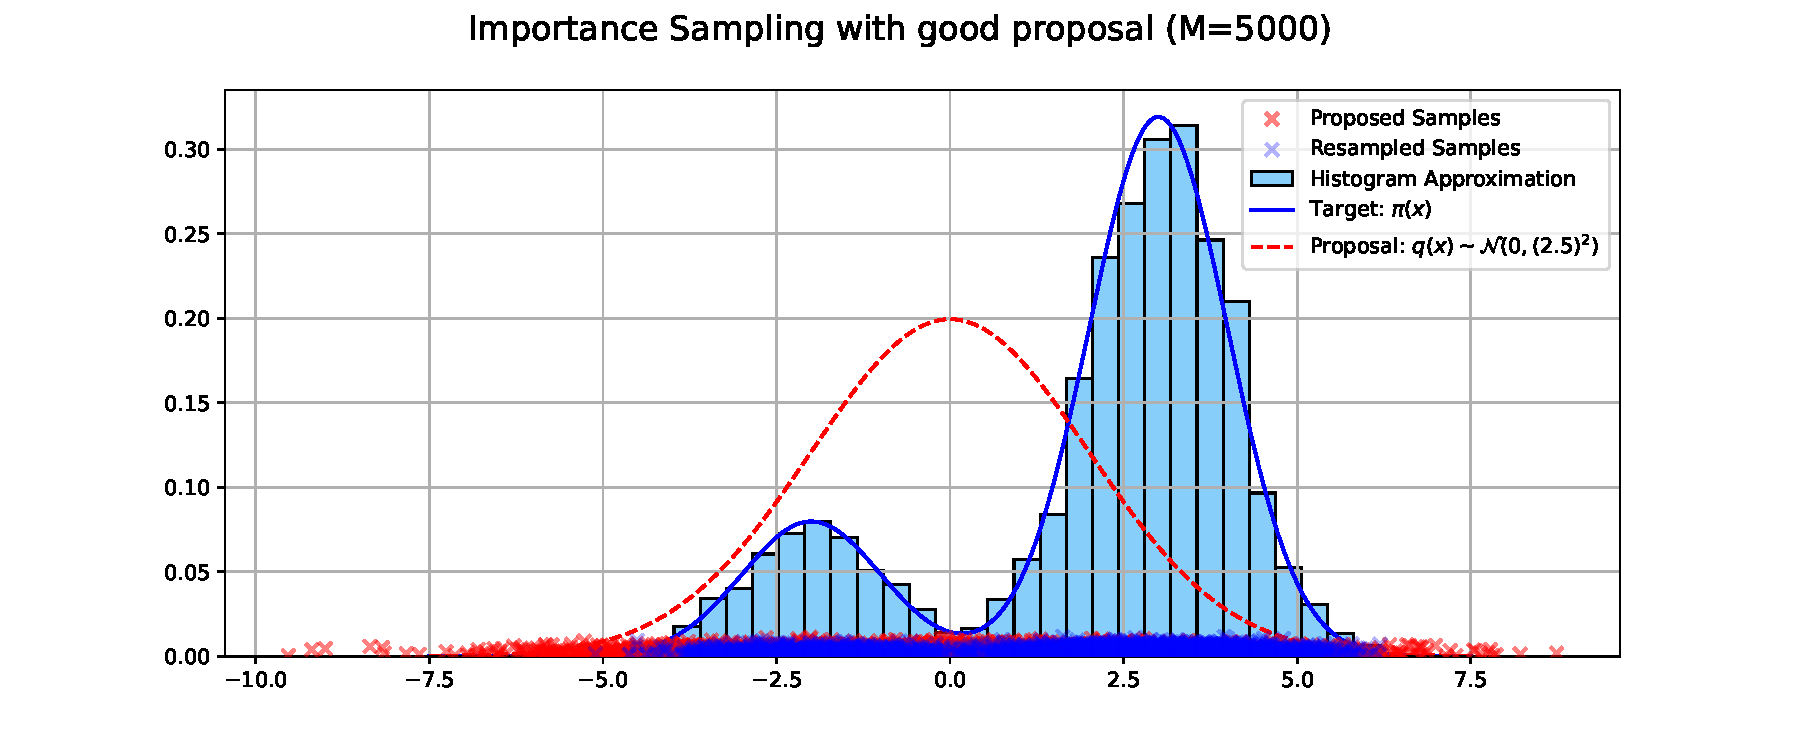
\includegraphics[scale=0.5]{pictures/IS_example1.pdf}
			    \caption{Approximation of a mixed Gaussian with $E[x] = 2$ using 5000 draws from a univariate normal distribution with good coverage. The histogram approximation accurately captures the two modes. The estimated mean $\hat{\mu} = 2.05$ is almost identical to the true value.}
			    \label{fig:IS_sim1}
			\end{figure}
			\vspace{0.5cm}
\end{frame}

\begin{frame}{Importance Sampling: Sample Size}
			\begin{figure}
			    \centering
			    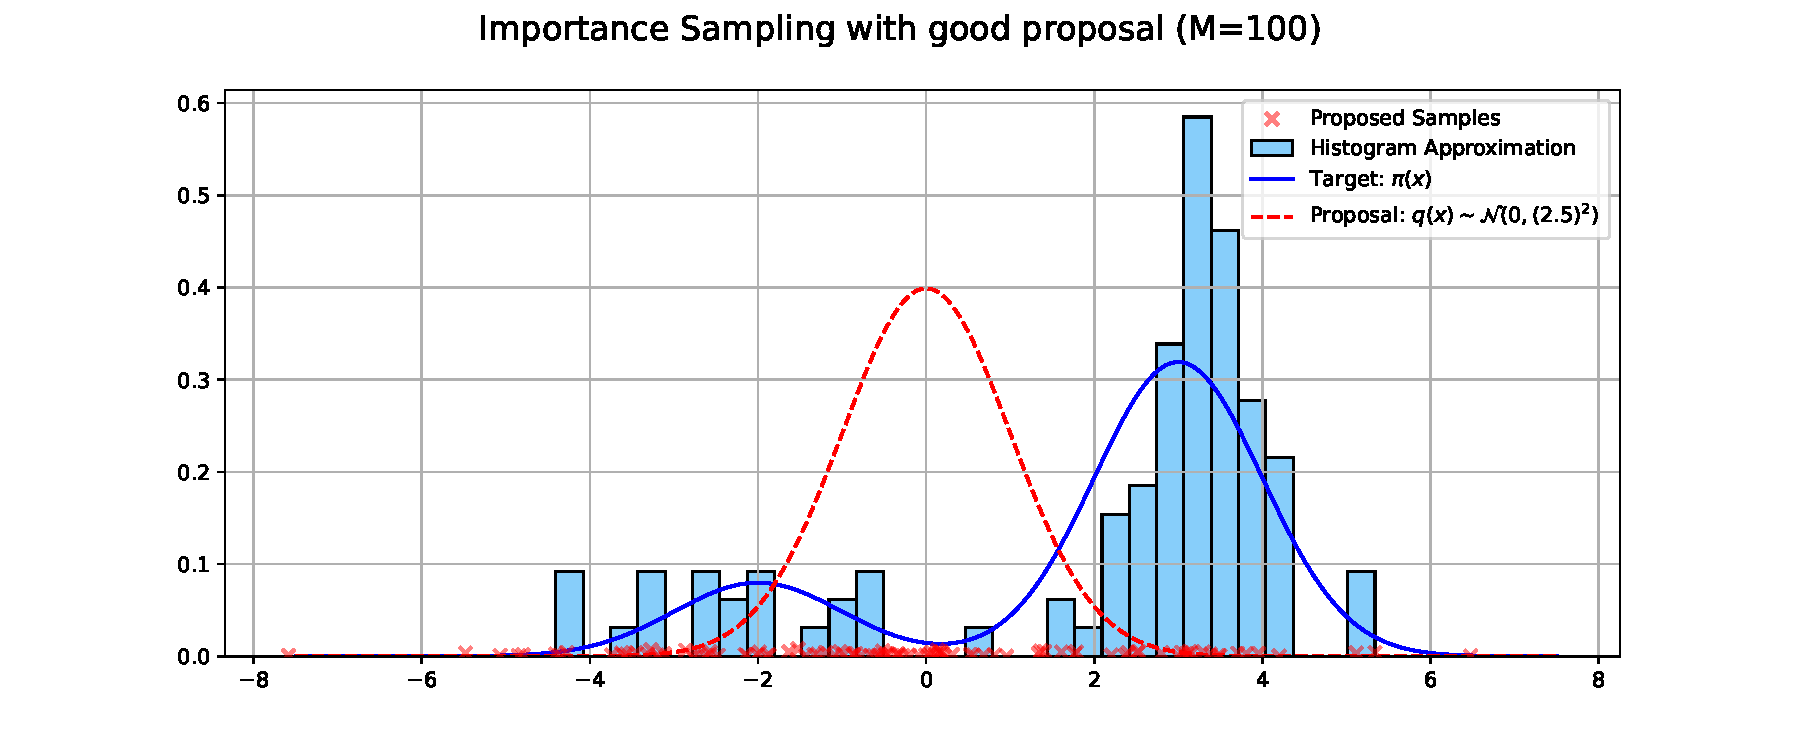
\includegraphics[scale=0.5]{pictures/IS_example3.pdf}
			    \caption{Approximation of a mixed Gaussian with $E[x] = 2$ using 100 draws from a univariate normal distribution. Due to low $M$ the histogram approximation is still sparse. However, with a value of $\hat{\mu} = 2.1$, the estimated mean is already close.}
			    \label{fig:IS_sim2}
			\end{figure}
			\vspace{0.5cm}
\end{frame}


\begin{frame}{Importance Sampling: Proposal Choice}
			\begin{figure}
			    \centering
			    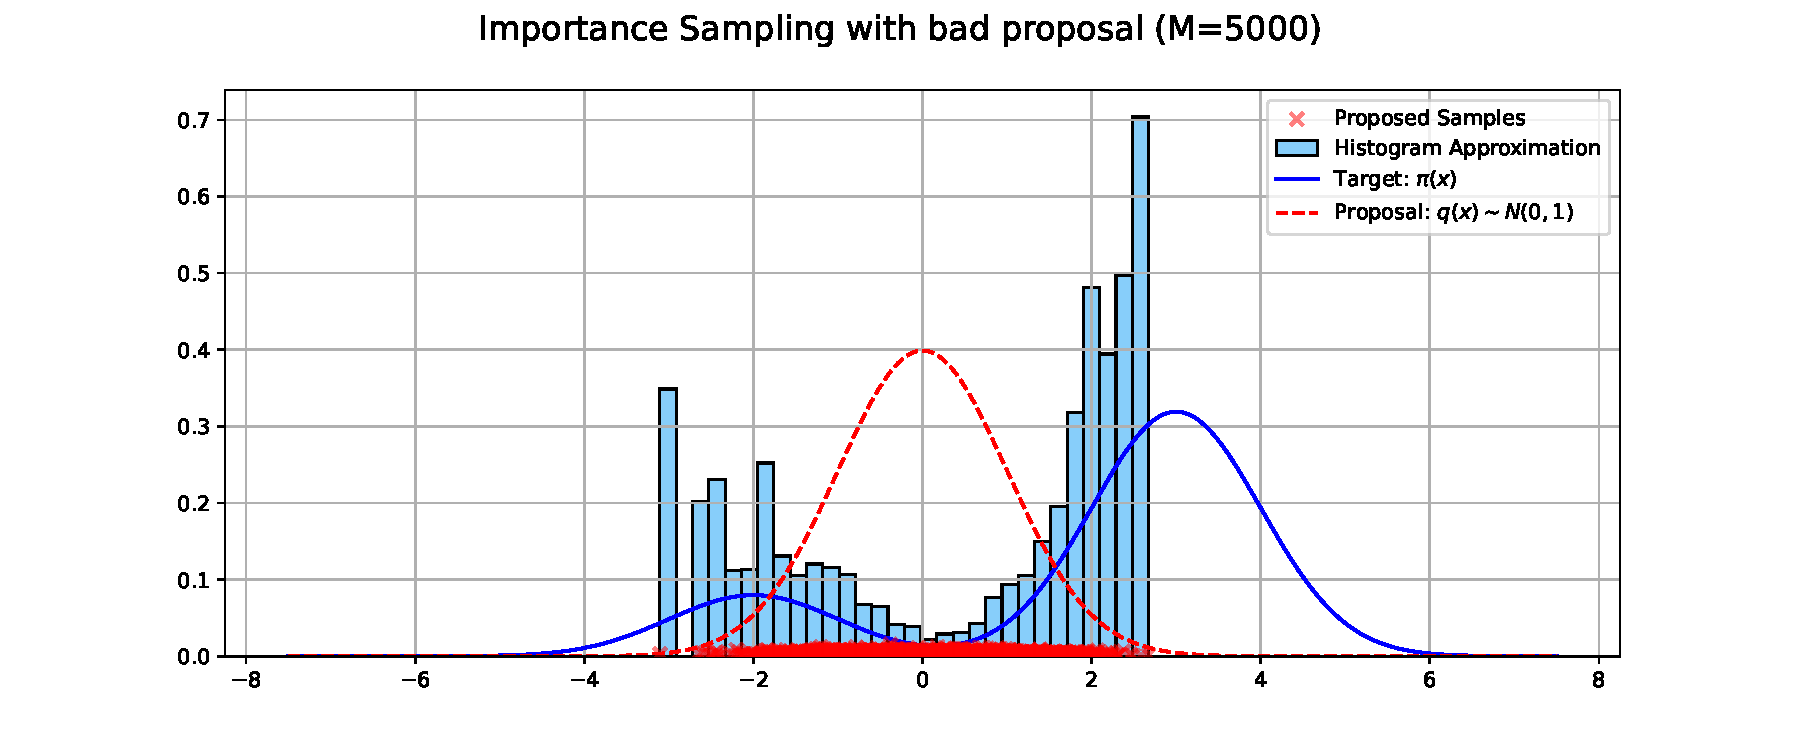
\includegraphics[scale=0.5]{pictures/IS_example2.pdf}
			    \caption{Example of a bad proposal that does not properly cover the modes of the target distribution. The histogram approximation can't capture the features of $\pi(x)$ well. Yet, the estimated mean $\hat{\mu} = 2.19$ is also not too far off.}
			    \label{fig:IS_sim3}
			\end{figure}
   \vspace{-0.3cm}
\begin{center}
    \textbf{How does the Sample Size and Proposal Choice affect the Accuracy of Importance Sampling?}
\end{center}
\end{frame}



\begin{frame}{Evaluating Estimation Accuracy of Importance Sampling}
\textbf{Simulation Set-up:}
\begin{itemize}
    \item Target Distribution: $\pi(x) \sim 0.8 \times \mathcal{N}(3, 1) + 0.2 \times \mathcal{N}(-2, 1)$ $\longrightarrow \mu=2, \sigma^2 = 4$
    \item Proposal Distributions: $q_1(x) \sim \mathcal{N}(0, (2.5)^2)$ and $q_2(x) \sim \mathcal{N}(0, 1)$
\end{itemize}
\textbf{Results for $N=1000$ Simulations and increasing sample size $M$:}
\begin{enumerate}
    \item Good Proposal ($q_1$):
    \begin{table}
        \centering
        \begin{tabular}{cccccc}
             \textbf{M} & \textbf{50} & \textbf{100} & \textbf{500} & \textbf{1000} & \textbf{5000} \\ \hline \hline
           Mean($\hat{\mu}$) & 1.956 & 1.935 & 1.989 & 2.007 & 2.001\\ 
           Var($\hat{\mu}$) & 0.26 & 0.14 & 0.025 & 0.012 & 0.003 \\ \hline
        \end{tabular}
        %\caption{Caption}
        \label{tab:my_label1}
    \end{table}
    \item Bad Proposal ($q_2$):
            \begin{table}[]
        \centering
        \begin{tabular}{cccccc}
            \textbf{M} & \textbf{50} & \textbf{100} & \textbf{500} & \textbf{1000} & \textbf{5000} \\ \hline \hline
           Mean($\hat{\mu}$) & 0.611 & 0.888 & 1.355 & 1.47 & 1.757 \\
           Var($\hat{\mu}$) & 1.445 & 1.319 & 0.761 & 0.596 & 0.305 \\ \hline
        \end{tabular}
        %\caption{Caption}
        \label{tab:my_label1}
    \end{table}
\end{enumerate}
\begin{center}
  \textbf{Estimates from $q_1(x)$ are far more precise with smaller variance (Factor of 100 for $M=5000$).}
\end{center}

\end{frame}

\begin{frame}{Empirical Applications:}
\textbf{Typical Applications in Economics}
\begin{enumerate}
    \item \cite{Herbst2014}: Approximate distribution of parameters of a dynamic macro model using Importance sampling
    \item \cite{Glasserman2005}: Analyze probabilities and risks of credit portfolios
    \item \cite {Doucet2001}: Analyze volatility in stock markets.
\end{enumerate}
\vspace{1cm}
\large{\textbf{In the application for the seminar paper we plan to use importance sampling to evaluate downside risks for the stock indices DAX and S\&P 500. }}
\end{frame}

\begin{frame}{Conclusion}
\textbf{Importance Sampling}
\begin{enumerate}
    \item ... provides a convinient methods to approximate Expectations when closed form solutions are hard/impossible to obtain
    \item ... conceptually simple and easy to implement on modern computers
    \item ... widely applicable to many econometric problems.
\end{enumerate}
\textbf{Drawbacks:} 
\begin{enumerate}
    \item Choice of correct proposal often not easy.
    \item Method becomes slow in high dimensions. 
\end{enumerate}
\textbf{Outlook:} 
\begin{enumerate}
\item Application of the method to evaluate credit risks.
\end{enumerate}

\end{frame}

\end{document}
